\documentclass[fleqn]{article}
\usepackage{graphicx}
\usepackage{amsmath,amsfonts,amssymb}
\usepackage{commath}

\usepackage{titlesec}
\titlelabel{\thetitle)\quad}

\usepackage{changepage,titlesec}
\titleformat{\section}[block]{\bfseries}{\thesection)}{1em}{}
\titleformat{\subsection}[block]{}{(\thesubsection)}{1em}{}
\titleformat{\subsubsection}[block]{}{(\thesubsubsection)}{1em}{}
\titlespacing*{\subsection} {2em}{3.25ex plus 1ex minus .2ex}{1.5ex plus .2ex}
\titlespacing*{\subsubsection} {4em}{3.25ex plus 1ex minus .2ex}{1.5ex plus .2ex}

\usepackage{geometry}
 \geometry{
 a4paper,
 total={170mm,257mm},
 left=20mm,
 top=20mm,
 }

\title{Homework 6}
\author{Submitted By: Puneet Singhal\\}
\date{}

\def\thesubsection{\alph{subsection}}
\def\thesubsubsection{\roman{subsubsection}}

\begin{document}
\maketitle
\pagenumbering{arabic}

\setcounter{section}{3}
\section{}
\begin{adjustwidth}{4em}{0pt}
	Output of layer 2 after 30 iterations is: \\
	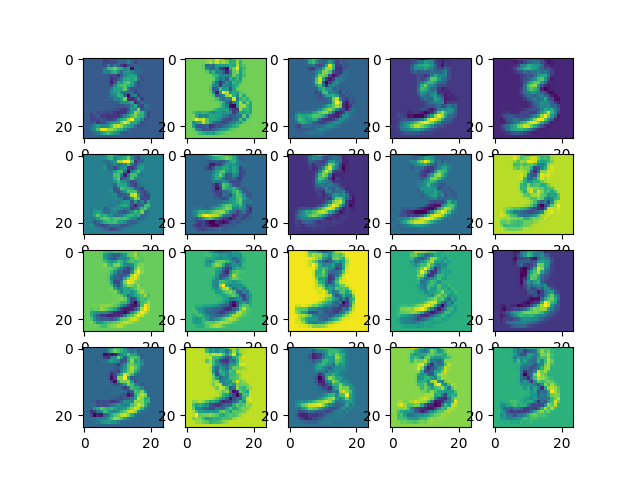
\includegraphics[scale = 1]{output2_30_iterations.png}\\ \\	
\end{adjustwidth}

\section{}
\begin{adjustwidth}{4em}{0pt}
	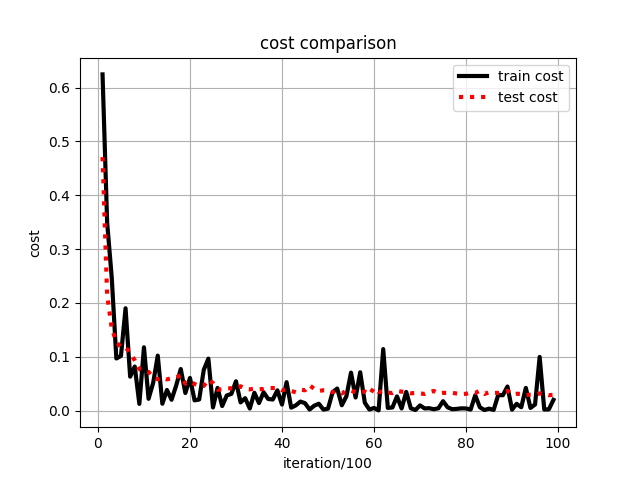
\includegraphics[scale = 1]{cost_comparison.png}\\ \\	
\end{adjustwidth}

\section{}
\begin{adjustwidth}{4em}{0pt}
	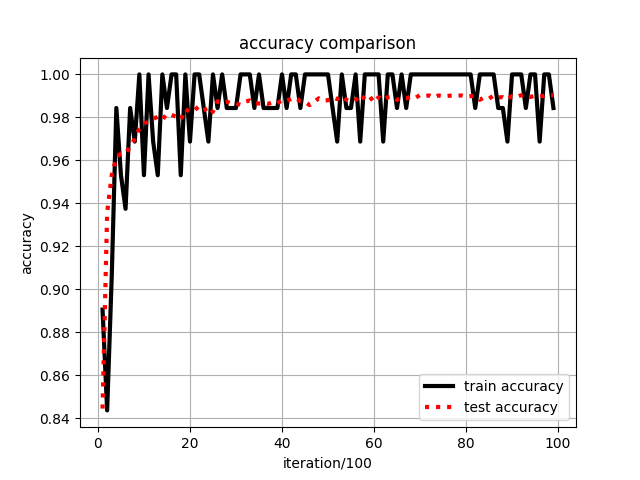
\includegraphics[scale = 1]{accuracy_comparison.png}\\ \\	
\end{adjustwidth}

\section{}
\begin{adjustwidth}{4em}{0pt}
	Test Accuracy = 99.03\%\\ 
	Time taken = 12381 seconds\\	
\end{adjustwidth}

\section{}
\begin{adjustwidth}{4em}{0pt}
	Output of layer 2 after 10000 iterations is: \\
	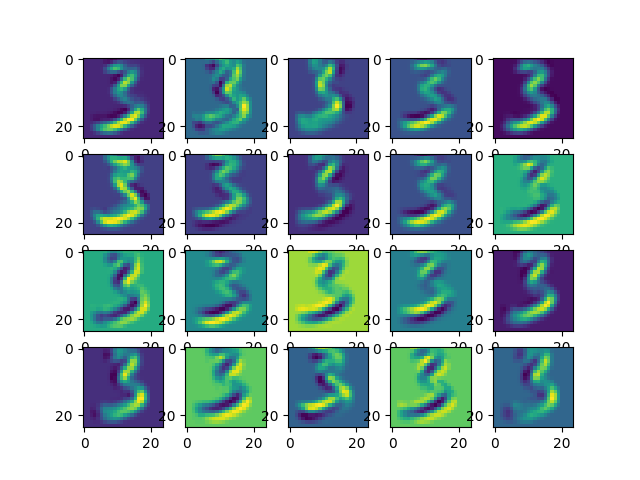
\includegraphics[scale = 1]{output2_10000_iterations.png}\\ \\	
\end{adjustwidth}

\section{}
\begin{adjustwidth}{4em}{0pt}
	After 10000 iterations, the weights have converged (deducted from stable accuracy and cost). Hence, we will expect clear information from the different neurons of convolution layer. This can be seen from comparing two images shown in Q4 and Q8. The features like yellow region in each output of convolution layer gives us information about the number in the image. In my case, the input image is number 3 and hence different outputs are highlighting different curves (lines) in number 3. In the output of convolution layer after 30 iterations, the features are not that clear and is very scattered.\\ \\	
\end{adjustwidth}

\section{}
\begin{adjustwidth}{4em}{0pt}
	Output of layer 2 after 10000 iterations is: \\
	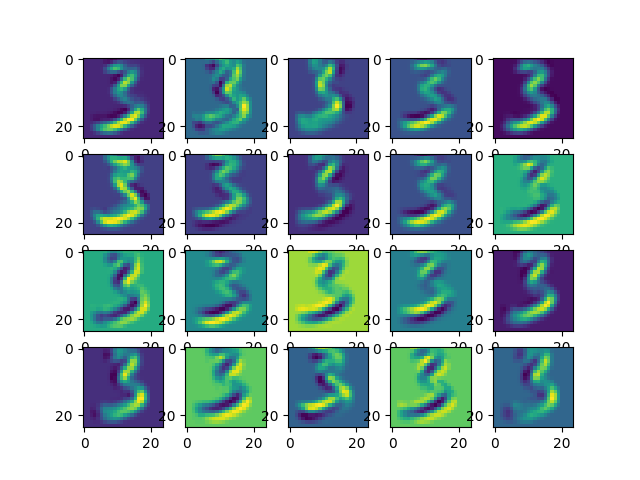
\includegraphics[scale = 1]{output2_10000_iterations.png}\\ \\
	Output of layer 3 after 10000 iterations is: \\	
	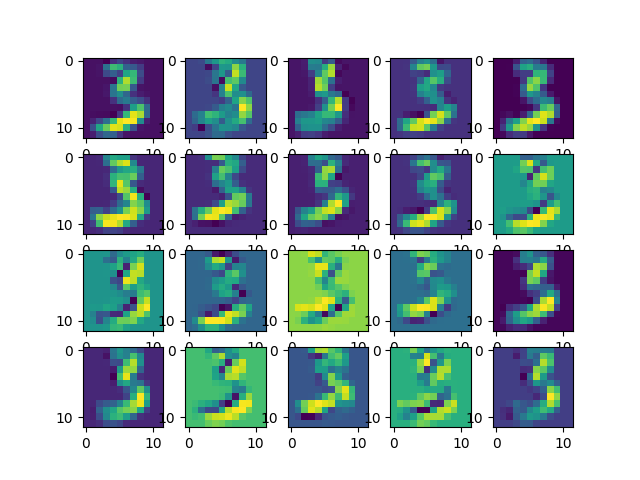
\includegraphics[scale = 1]{output3_10000_iterations.png}\\ \\	
\end{adjustwidth}

\section{}
	Original image is:	 \\ \\
	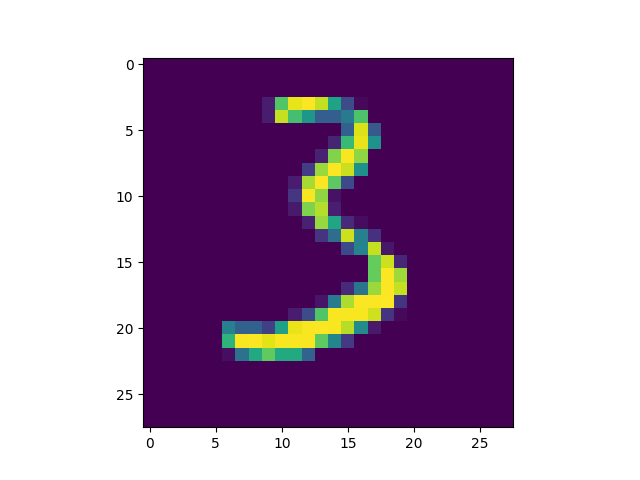
\includegraphics[scale = 1]{original_image.png}\\ 
\subsection{}
	\begin{adjustwidth}{4em}{0pt}
		In the original image, the number 3 is visible with yellow region in the middle of lines/curves and blue shade on the outside, constructing the number. After 10000 iterations, convolution layer is able to extract this information by extracting different segments as different outputs. Looking at these features in different outputs of convolution layer, we can infer that the number is indeed 3. \\	
	\end{adjustwidth}

\subsection{}
	\begin{adjustwidth}{4em}{0pt}
		At the output of 3rd layer (Max pool layer), the features are clear even with smaller number of pixels. This can be seen from the images where the different output still contain the same information about the features. This helps us decrease the dimensions without compromising on the predictions. \\	
	\end{adjustwidth}
	
\section{}
\begin{adjustwidth}{4em}{0pt}
	No \\	
\end{adjustwidth}

\section{}
\begin{adjustwidth}{4em}{0pt}
	No \\	
\end{adjustwidth}

\section{}
\begin{adjustwidth}{4em}{0pt}
	No \\	
\end{adjustwidth}

\end{document}